
\section{Programação Genética}
\label{cap::gp}

No Capítulo~\ref{cap::metodo},
além de mostrarmos os algoritmos de classificação \textit{Naïve Bayes} e \textsc{KNN}, vimos como podemos incorporar a credibilidade nos mesmos.
Discutimos também que existem várias métricas que podem ser utilizadas para mensurar a credibilidade de um exemplo, 
embora não detalhamos essas métricas.

Nesse trabalho, modelamos a credibilidade em duas abordagens diferentes, uma levando em consideração os atributos dos exemplos e outra utilizando os seus relacionamentos. 
Em ambas, somos capazes de gerar uma grande gama de métricas que conseguem capturar a relação entre os exemplos e uma determinada classe.
Entretanto, necessitamos de uma forma de selecionar e combinar essas métricas de uma maneira robusta. Para solucionar esse problema, recorremos ao uso de Programação Genética (\textsc{PG}).

Segundo a Teoria da Evolução de Darwin, indivíduos mais adaptados ao ambiente em que se encontram têm uma maior chance de sobreviverem e se reproduzirem, passando seu material genético às gerações posteriores. Baseado nessa teoria, o método Programação Genética é adequado para evoluir uma função de credibilidade, pois possui mecanismos que o torna capaz de explorar bem o imenso espaço de soluções formado pelo grande número de métricas disponíveis. Além disso, \textsc{PG} é flexível o bastante para podermos representar as funções que desejamos.
%Programação Genética é um método baseado na Teoria da Evolução de Darwin que define que indivíduos mais adaptados ao ambiente em que se encontram têm uma maior chance de sobreviverem e se reproduzirem, passando seu material genético às gerações posteriores. PG é um método adequado para evoluir uma função de credibilidade, pois consegue explorar bem o imenso espaço de soluções formado pelo grande número de métricas disponíveis e é flexível o bastante para podermos representar as funções que desejamos.

Para entendermos melhor como é o funcionamento de um \textsc{PG}, a Figura~\ref{fig::gpwf} ilustra de forma genérica os seus principais componentes.
Como podemos ver, o primeiro passo é definirmos um conjunto de funções internas e terminais para serem usados pelo \textsc{PG}, iremos explicar com mais clareza e exemplos o que são funções internas e terminais em breve nesse capítulo, porém é importante saber agora que eles são usados para formarmos indivíduos. 
Esses por sua vez são soluções para o problema que abordamos (em nosso caso, um indivíduo é uma possível função de credibilidade).
Um conjunto de indivíduos é chamado de população e, como mostrado pelo segundo retângulo no diagrama da Figura~\ref{fig::gpwf}, a população inicial é aleatoriamente criada. 
Cada indivíduo é então avaliado por uma função de \textit{fitness}, que calcula a habilidade do mesmo em resolver o problema apresentado, ou seja, o quão bom aquele indivíduo é.

Após avaliarmos a \textit{fitness} dos indivíduos, os melhores são selecionados e submetidos às operações genéticas de cruzamento, mutação e reprodução, com probabilidade $P_c$, $P_m$ e $P_r$, respectivamente.
Uma forma muito usada de selecionar os indivíduos é através de torneios, nos quais aleatoriamente tomamos um número pré-definido de indivíduos da população e selecionamos aquele com maior valor da função de \textit{fitness}. Existem diversas outras variações do método de seleção, ver (citacao), sendo que o importante é utilizarmos o conhecimento da função \textit{fitness} dos indivíduos de forma a criamos uma próxima geração mais bem preparada para resolução do problema. 

Após selecionados, os indivíduos podem sofrer alguma alteração genética através das operações de mutação e cruzamento ou podem ser transferidos diretamente para a próxima geração, através da reprodução. 
Na operação de mutação, uma parte do indivíduo selecionado é aleatoriamente alterada, buscando obter uma melhoria da \textit{fitness} na próxima geração.
Por sua vez, a operação de cruzamento exige a participação de dois indivíduos que são combinados a fim de obtermos uma prole mais adaptada na próxima geração.
Do modo como está mostrado na Figura~\ref{fig::gpwf} somente uma dessas três operações é realizada em cada indivíduo selecionado, entretanto é comum também implementações em que é aplicada a probabilidade de mutação para todos os indivíduos, logo após uma nova prole ser gerada pelo cruzamento ou reprodução.

Repare que todo o \textit{processo} exposto na Figura~\ref{fig::gpwf} é independente da aplicação na qual o \textsc{PG} é utilizado. 
Entretanto, três importantes componentes devem ser instanciados dependendo do contexto no qual trabalhamos. 
Eles são a representação dos indivíduos, que incluem as funções internas e terminais utilizados (Seção~\ref{subsec::individuos}), a função de \textit{fitness} (Seção~\ref{subsec::fitness}) e como são usados os operadores genéticos (Seção~\ref{subsec::operadores}).

\begin{figure}[ht!]
\centering
\includegraphics[width=1.0\textwidth]{figures/gpwf.png}
\caption{Fluxograma de um Programa Genético}
\label{fig::gpwf}
\end{figure}

\subsection{Indivíduos}
\label{subsec::individuos}

Uma parte essencial da construção um \textsc{PG} é definir os indivíduos que compõem a população do mesmo.
Para isso, temos que ter definir três aspectos primordiais, o que um indivíduo representa, quais serão suas funções internas e quais são os seus terminais. Independente de quais são as funções internas e terminais escolhidos, o propósito de um indivíduo é representar uma função de credibilidade que, a não ser que seja dito o contrário, relaciona um exemplo de treino a uma classe retornando um valor real. 

Como já discutido nas Seções~\ref{subsubsec::nbcredconteudo} e \ref{subsubsec::nbcredgrafos} para o \textit{Naïve Bayes} e Seções~\ref{subsubsec::knncredconteudo} e \ref{subsubsec::knncredgrafos} para o \textsc{KNN}, modelamos duas funções de credibilidade diferentes, uma baseada nos atributos dos exemplos e outra baseada nos relacionamentos dos mesmos.
Ambas, entretanto, compartilham o mesmo conjunto de funções internas, porém os terminais utilizados são diferentes para cada caso. As funções internas são utilizadas para que haja uma interação entre os terminais.
Como usual para um \textsc{PG} que evolui uma função matemática numérica, as funções internas do \textsc{PG} consistem de funções matemáticas conhecidas, como a multiplicação, divisão, soma entre outros que estão mostrados na Tabela~\ref{table::funcoespg}. 
Observe que modificações as funções de subtração, divisão e logaritmo.
Tanto a divisão por zero, quanto o logaritmo de números negativos não são matematicamente definidos, portanto explicitamente tratamos esses casos retornando zero. Além disso, não queremos ter uma função de credibilidade negativa, portanto evitamos que a subtração e o logaritmo retornem números negativos.

\begin{table}[ht*]
\centering
\begin{tabular}{|c|c|}
\toprule
    \textbf{Função Interna} & \textbf{Explicação} \\
\midrule
    $+(a,b)$           & Soma a com b. \tabularnewline \hline
    $-(a,b)$           & Subtrai b de a, porém retorna 0 se b for maior que a.\tabularnewline \hline
    $\times(a,b) $     & Multiplica a com b. \tabularnewline \hline
    $\%(a,b)$          & Divide a por b, porém retorna 0 se b for 0. \tabularnewline \hline
    $\text{Pow}(a,b)$  & Eleva à potência de b. \tabularnewline \hline 
    $\log(a,b) $       & Logaritmo de a na base b, retorna 0 se a ou b forem menores que 1. \tabularnewline
\bottomrule
\end{tabular}
\caption{Explicação das principais funções utilizadas para definição das métricas para atributos textuais.}
\label{table::funcoespg}
\end{table}

Pelo fato de termos um grande número de operadores definidos, reservamos as Seções~\ref{sec::pg_cred_baseada_conteudo} e~\ref{sec::pg_cred_baseada_grafos} exclusivamente para descrevermos os operadores relacionados ao atributos dos exemplos e em mensurar os relacionamentos entre os exemplos, respectivamente. Na Figuras~\ref{fig::gps1} e~\ref{fig::gps2} temos ao todo cinco exemplos de funções de credibilidades que poderiam ser geradas pelo \textsc{PG}, as três da primeira figura ilustram funções de crebilidade baseadas em atributos e as demais são baseadas em relacionamentos entre os exemplos. As cores nas mesmas são usadas apenas para auxiliar na explicação das operações genéticas de mutação e cruzamento na seção a seguir.

\begin{figure}[ht]
\centering
\subfloat[Individuo 1:\newline \hspace*{6mm}$\textsc{GINI}(x)^{\textsc{CC}(x,c)}$]{
    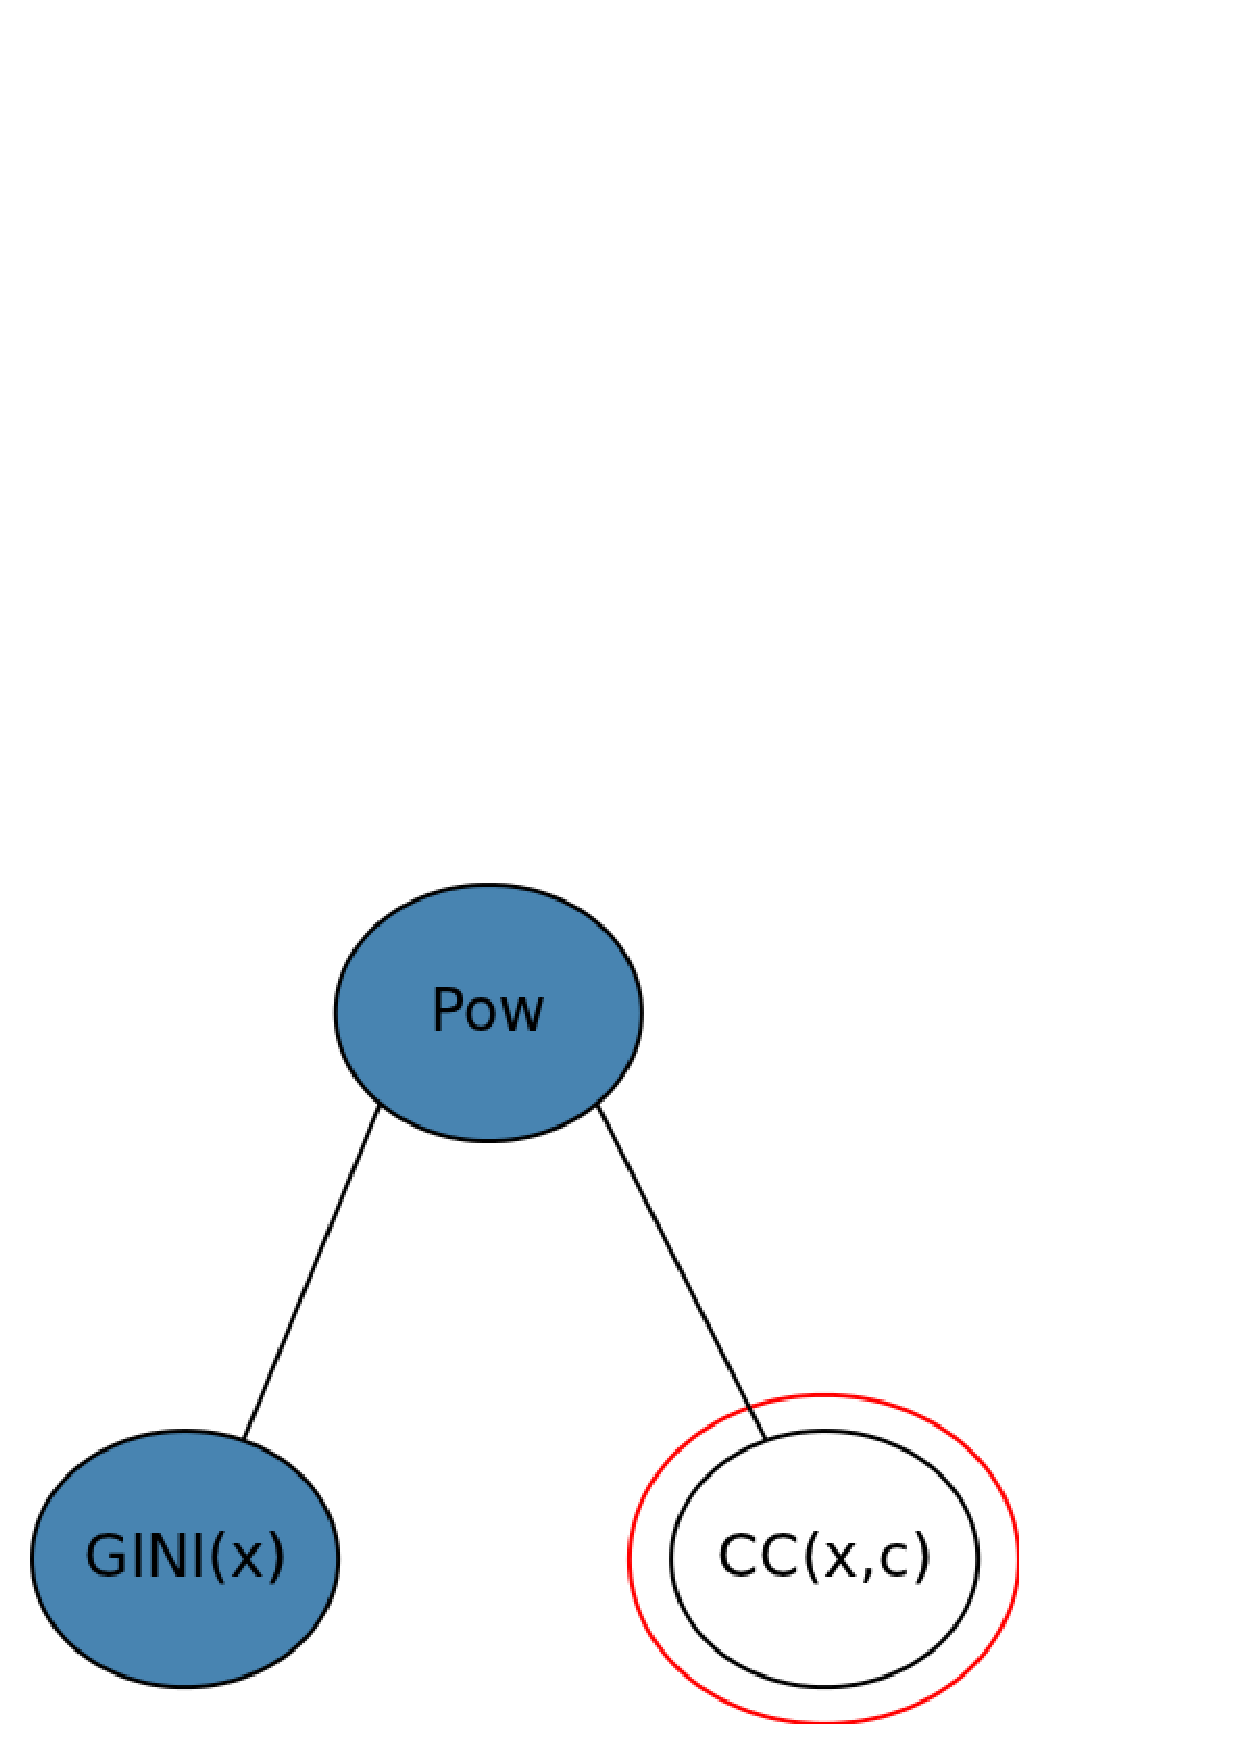
\includegraphics[width=0.25\textwidth]{figures/gp1c.png}
}
\subfloat[Individuo 2:\newline \hspace*{4mm} $(\textsc{AM}(x,c) + \textsc{P}(x|c)) \% (\textsc{IG}(x,c))$]{
    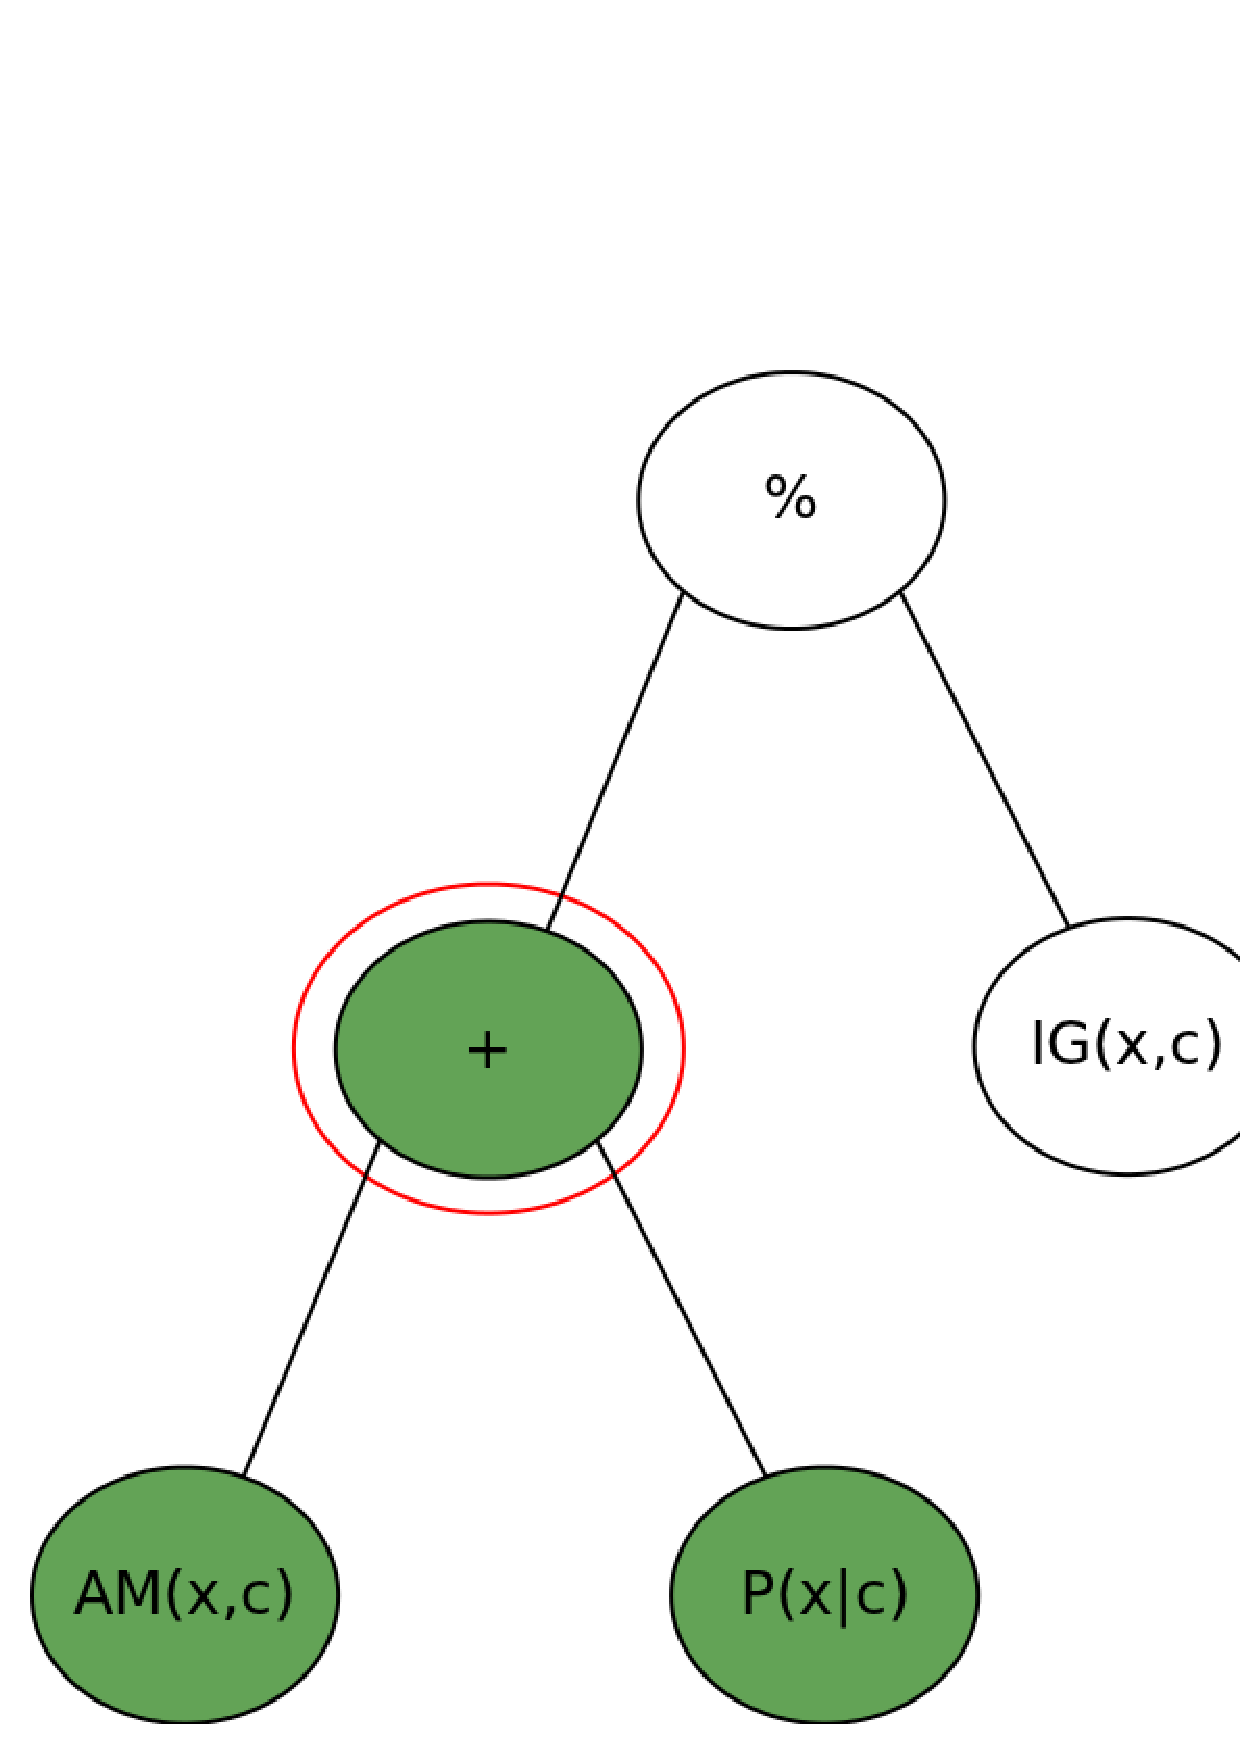
\includegraphics[width=0.33\textwidth]{figures/gp2c.png}
}
\subfloat[Individual 3:\newline \hspace*{4mm} $\textsc{GINI}(x)^{(\textsc{AM}(x,c)\ + \ \textsc{P}(x|c))}$]{
    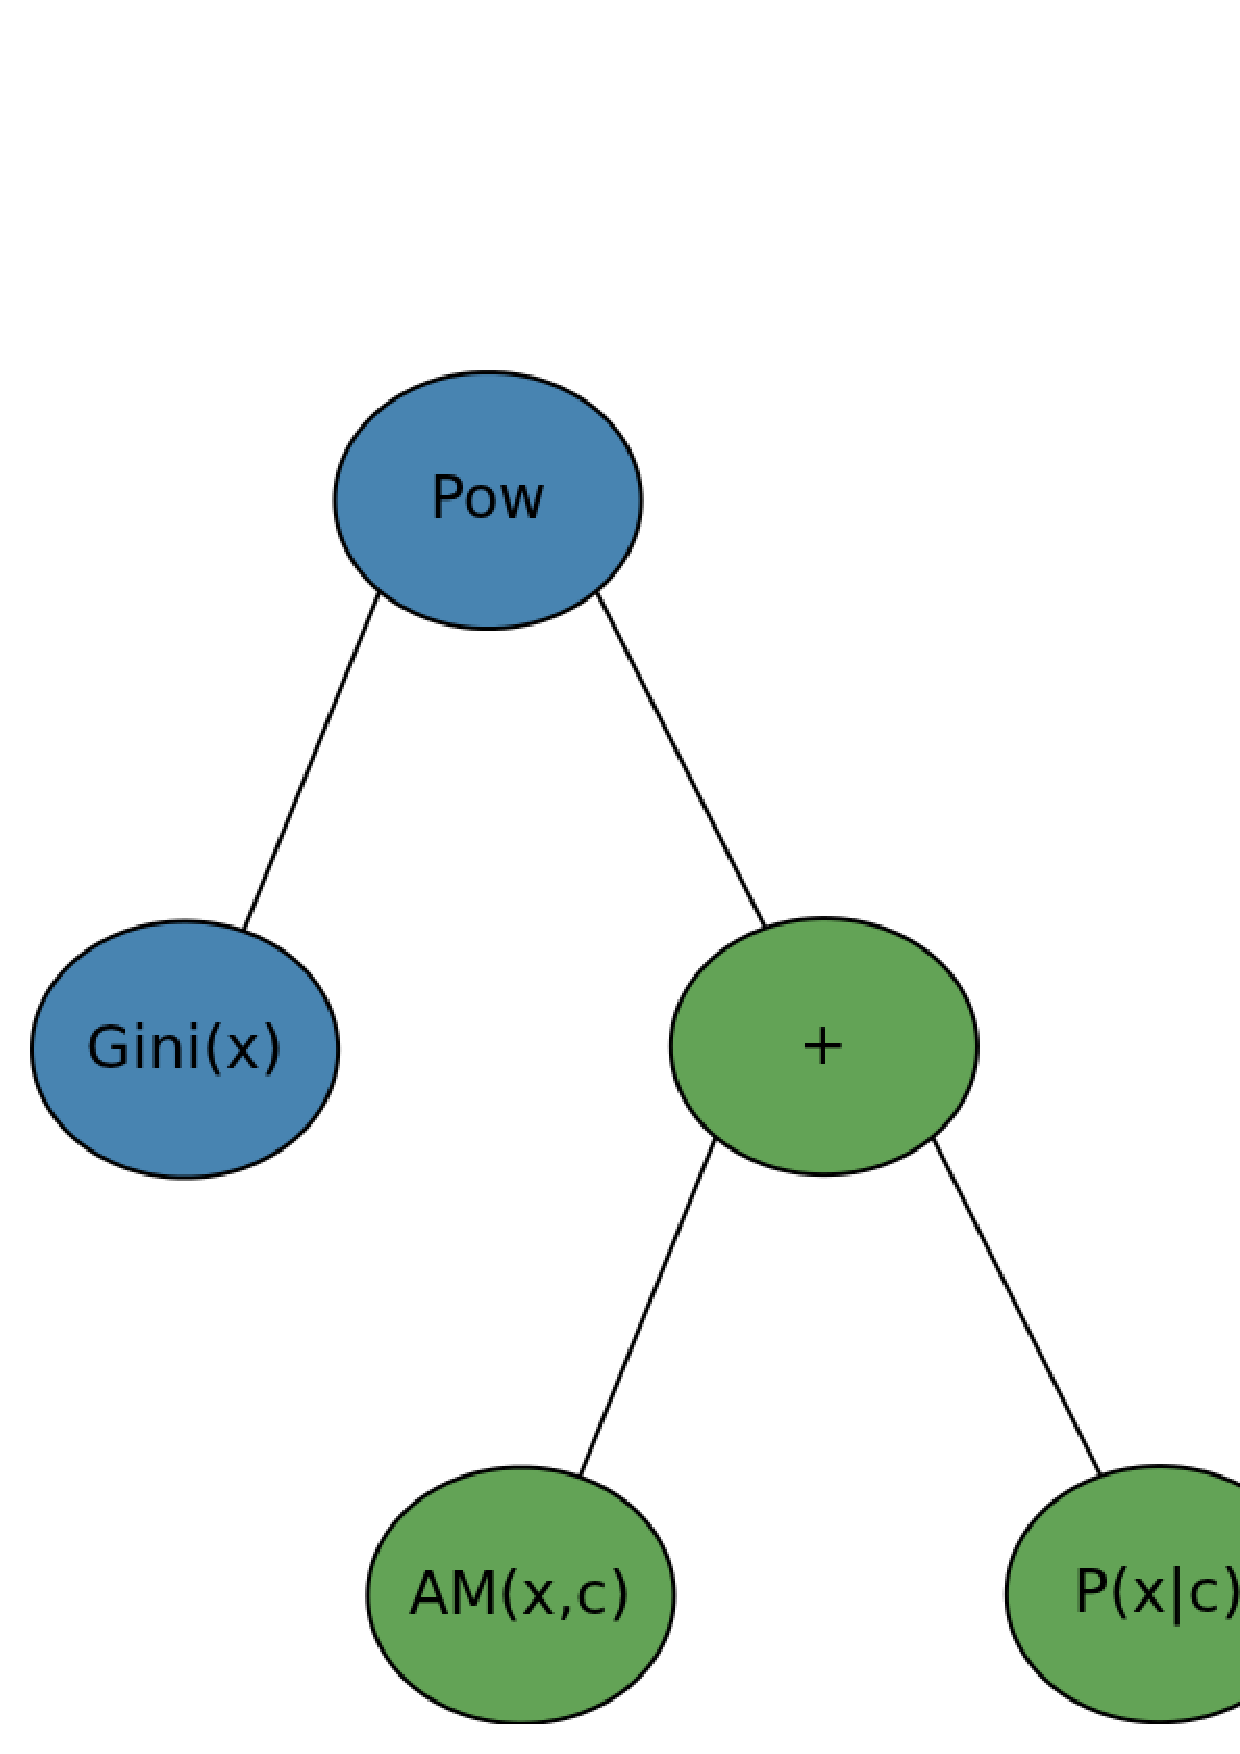
\includegraphics[width=0.33\textwidth]{figures/gp3c.png}
}
\caption{Três possíveis indivíduos utilizados como função de credibilidade de atributos.}
\label{fig::gps1}
\end{figure}


\begin{figure}[ht]
\centering
\subfloat[Individuo 1:\newline \hspace*{6mm}$\textsc{Bib}(X,c) - {\textsc{Hub}(x,c)}$]{
%\subfloat[Individuo 1:$\textsc{Bib}(X,c) - {\textsc{Hub}(x,c)}$]{
    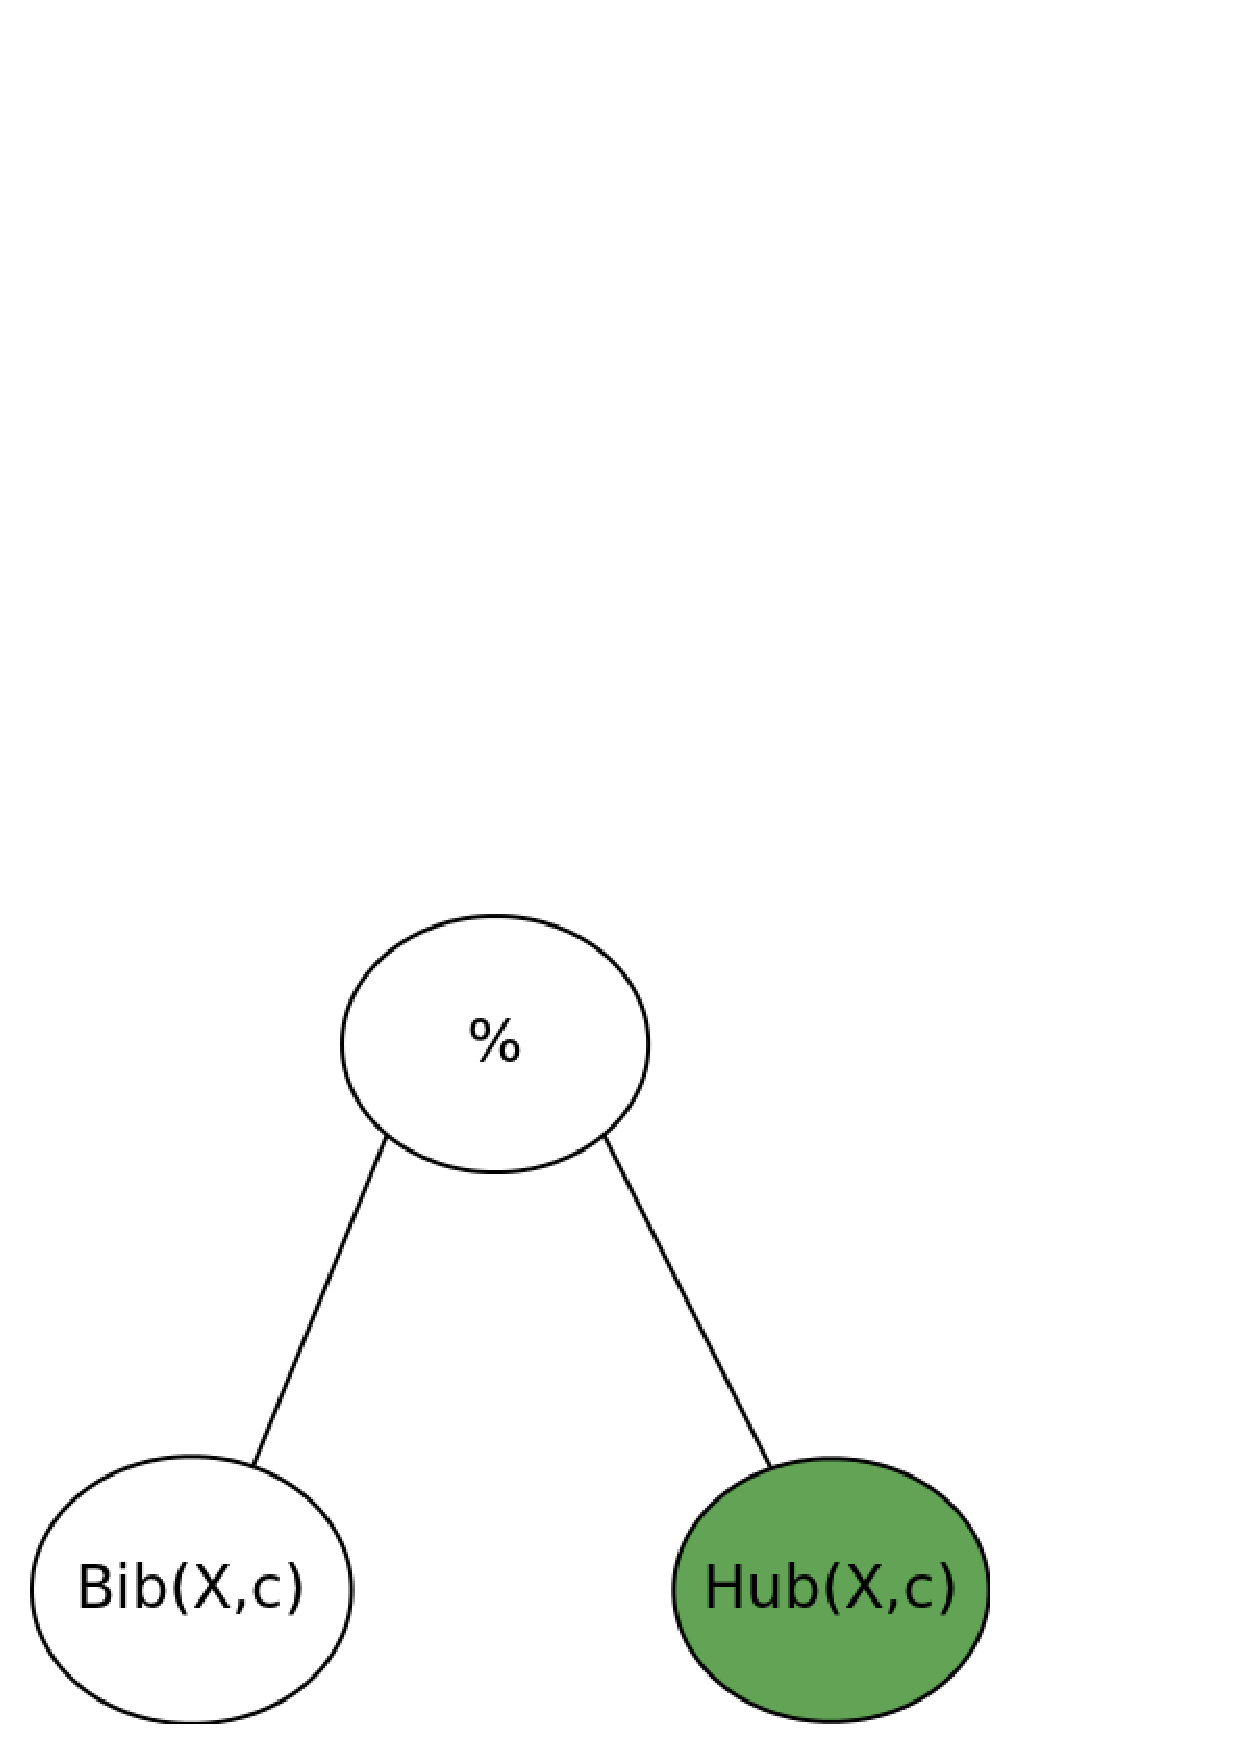
\includegraphics[width=0.30\textwidth]{figures/gp1c_grafos.png}
}
\subfloat[Individuo 2:\newline \hspace*{5mm} $\textsc{Bib}(X,c) - \textsc{PR}(X,c) $]{
    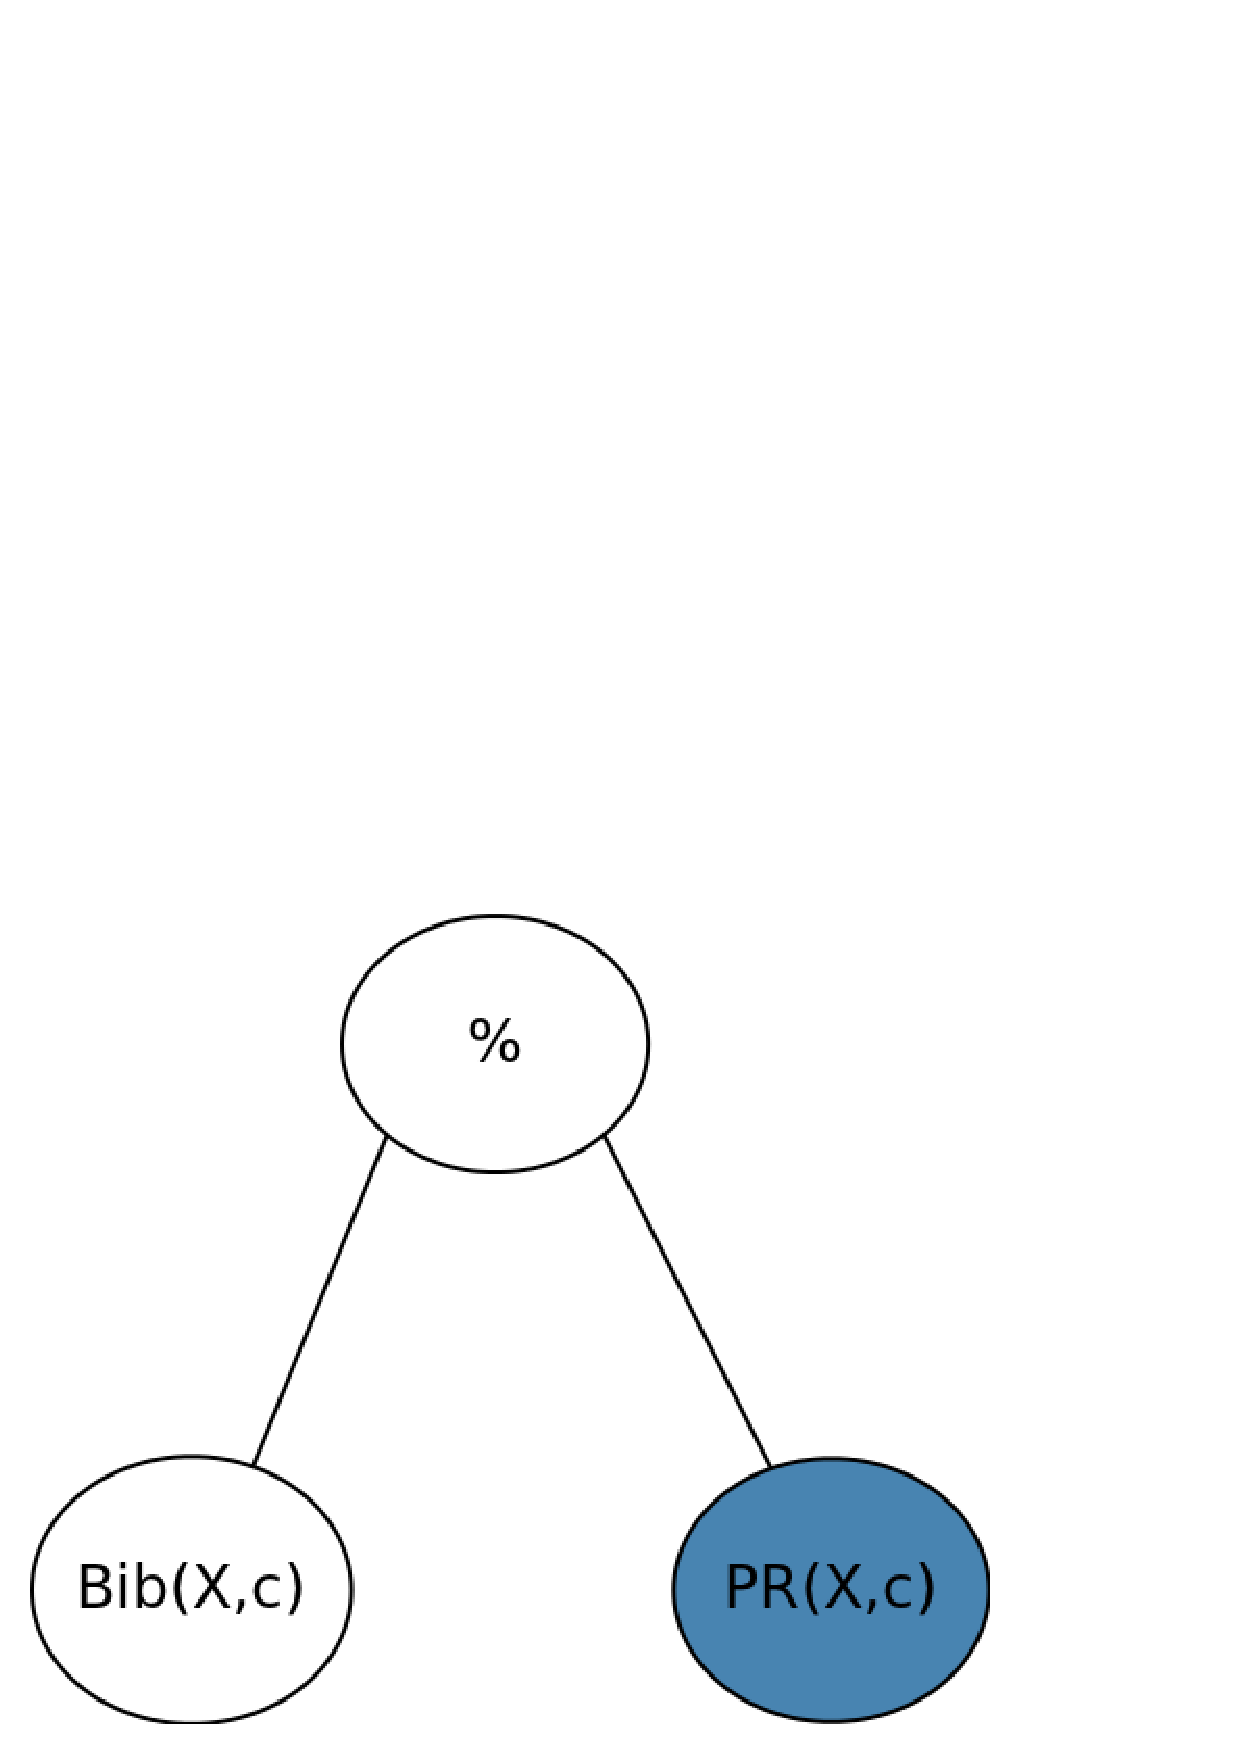
\includegraphics[width=0.30\textwidth]{figures/gp2c_grafos.png}
}
\caption{Dois possíveis indivíduos utilizados como função de credibilidade para relacionamentos.}
\label{fig::gps2}
\end{figure}

\subsection{Operadores Genéticos}
\label{subsec::operadoresgeneticos}

Em nosso trabalho, utilizamos três operadores genéticos na geração dos indivíduos, como mostrado na Figura~\ref{fig::gpwf}. Primeiramente, sorteamos teremos uma operação de cruzamento, mutação ou reprodução, para o primeiro caso, sorteamos dois indivíduos, para os demais casos, apenas um. Os indivíduos são selecionados por torneio, onde escolhemos aleatoriamente $T$ indivíduos da população atual e dizemos que aquele com maior \textit{fitness} é o ganhador do torneio. 

A operação de reprodução é a mais simples, nela apenas introduzimos o ganhador do torneio na próxima geração. Por sua vez, a operação de cruzamento é a mais complexa. Nela selecionamos um ponto em cada indivíduo e geramos um novo indivíduos contendo partes de ambos. Na Figura~\ref{fig::gps1}, temos a ilustração desse processo. 
Os indivíduos 1 e 2 são selecionados cada um por um torneio diferente, depois escolhemos um ponto de troca no indivíduo 1, no caso a métrica \textsc{CC(x,c)} e um ponto de troca no 2, a função interna +. Por fim, trocamos a métrica \textsc{CC(x,c)} por toda a parte selecionada no indivíduo 2, gerando o indivíduo 3. Finalmente, a operação de mutação também consiste em uma troca em um indivíduo, porém trata-se de apenas uma única mudança, sem alterar a estrutura. Na Figura~\ref{fig::gps2} vemos uma mutação ocorrendo entre o indivíduo 1 e 2, onde temos a métrica Hub (Seção~\ref{subsubsection::hub}) sendo trocada pela métrica \textit{PageRank} (\textsc{PR}, Seção~\ref{subsubsection::pagerank}).


\subsection{\textit{Fitness}}
\label{subsec::fitness}

No algoritmo~\ref{alg::fitness} descrevemos o processo usado para calcular a \textit{fitness} de um individuo. 
Mesmo existindo casos em que estamos interessados somente em evoluir uma função de credibilidade, ou atributos ou relacionamentos, o algoritmo~\ref{alg::fitness} aborda ambos os casos. 
Quando não estivermos evoluindo uma das funções de credibilidade, basta ignorá-la no calculo da \textit{fitness}.
No algoritmo~\ref{alg::fitness}, primeiramente calculamos e mapeamos a credibilidade de cada atributo e cada classe para a função de credibilidade que o individuo representa. Logo depois, calculamos a credibilidade de cada relacionamento no conjunto de relacionamentos $\mathbb{R}$, usando o conjunto de exemplos $\mathbb{E}$ do treinamento.
Por fim, calculamos qual o valor da métrica chamada \textit{$F_1$} para os resultados do classificador utilizado. 
O classificador recebe o conjunto de exemplos de teste, $\mathbb{T}$, o conjunto de exemplos de treinamento, $\mathbb{E}$, o conjunto de classes, $\mathbb{C}$ e os valores mapeados para as funções de credibilidade de atributos e relacionamentos, $f_x$ e $f_r$.

A \textit{$F_1$} é uma métrica amplamente utilizada por representar um compromisso interessante entre a precisão e a revocação, outras duas importante métricas. A precisão ($\textsc{P}$) calcula, para uma classe específica, o quanto acertamos entre todos os exemplos que classificamos para aquela classe: 
\begin{equation}
\textsc{P(c)} = \frac{\# \text{de exemplos da classe c corretamente classificados como classe c}} {\# \: \text{ total de exemplos classificados como classe c}} \\,
\end{equation}
logo determinamos o quão bom somos em avaliar exemplos de uma classe específica. 
Por sua vez, a revocação (\textsc{R}) calcula, para uma classe, o quanto conseguimos acertar entre o que deveríamos ter acertado:
\begin{equation}
\textsc{R(c)} = \frac{\# \: \text{de exemplos da classes c corretamente classificados como classe c}}{\# \: \text{de exemplos existentes na classe c}},                      
\end{equation}
logo, calculamos o quão bom somos para achar exemplos de uma dada classe. 
Por fim, a \textit{$F_1$} é a média harmonica entre a precisão e a revocação:
\begin{equation}
\text{F}_1(c) = \frac{2 \times P(c) \times R(c)}{(P(c) + R(c))}.
\end{equation}

A partir da $F_1$ podemos calcular as métricas \textit{macro-$F_1$} e \textit{micro-$F_1$}. A \textit{macro-$F_1$} leva em consideração a $F_1$ de cada uma das classes e depois calcula a média das mesmas:
\begin{equation}
\text{MacroF}_1 = \frac{\sum\limits_{c \in \mathbb{C}} F_1(c) } { |\mathbb{C}| },
\end{equation}
já a \textit{micro-$F_1$} simplesmente calcula a precisão e revocação ao final, sem levar em consideração o cálculo classe por classe. Decidimos por utilizar a \textit{micro-$F_1$} como função de \textit{fitness} pelos bons resultados encontrados, porém sempre medimos e reportamos a \textit{macro-$F_1$}. Mostramos os resultados dos vários experimentos com micro e macro-F1, além de uma combinação de ambas no Capítulo~\ref{cap::experimentos}.

%traduzir comandos?!?!
\algrenewcommand\algorithmicforall{\textbf{Para Cada}}
\algrenewcommand\algorithmicdo{\textbf{Faça}}
\algrenewcommand\algorithmicfunction{\textbf{Função}}
\algrenewcommand\algorithmicreturn{\textbf{retorna}} %% nao sei pq nao funciona, pesquisar depois

\begin{algorithm}
\centering
\caption{Calula Fitness.}
\label{alg::fitness}
\begin{algorithmic}[1]
{
%\scriptsize
\Function{CalculaFitness}{$individuo$}
  \State \textit{Credibilidade baseada em atributos:}
  \ForAll{$x \in \mathbb{A}$}
    \ForAll{$c \in \mathbb{C}$}
      \State $f_a(x,c) \gets eval(individuo_{attrs}, x, c)$
    \EndFor
  \EndFor
  \State \textit{Credibilidade baseada em relacionamentos:}
  \ForAll{$r \in \mathbb{R}$}
    \ForAll{$e \in \mathbb{E}$}
        \ForAll{$c \in \mathbb{C}$}
            \State $f_r(r,d,c) \gets eval(r,individuo_{rel}, d, c)$
        \EndFor
    \EndFor
  \EndFor
  \State \textit{Avaliação da Fitness:}
  \State fitness $\gets$ \textsc{F$_1$}(\textsc{Classifier}$(\mathbb{T}, \mathbb{E}, \mathbb{C}, f_x, f_r)$)
  \State \textbf{return} fitness
\EndFunction
}
\end{algorithmic}
\end{algorithm}

\section{Credibilidade baseada no Conteúdo}
\label{sec::pg_cred_baseada_conteudo}

Nessa seção apresentamos várias métricas utilizadas na construção dos indivíduos usados pelo Programa Genético. Elas foram modeladas diferentemente para os casos nos quais os atributos são textuais ou categóricos, sendo que a modelagem para atributos numéricos foi deixada como trabalho futuro. Em suma, métricas que realizam cálculos baseados em frequência de termos e documentos não puderam ser usadas para atributos categóricos, porém todas as demais foram. Dessa forma, na Seção~\ref{subsec::pg_metricas_conteudo_textual} temos as métricas que foram modeladas única e exclusivamente para serem utilizadas na tarefa de classificação de textos e na Seção~\ref{subsec::pg_metricas_conteudo} temos as métricas que foram estendidas e estão sendo usadas para classificação categórica, além da textual.

\subsection{Métricas Modeladas Para Atributos Textuais Exclusivamente.}
\label{subsec::pg_metricas_conteudo_textual}

As métricas usadas para atributos textuais consistem em algumas variantes do \textsc{TFIDF}, métrica mais difundida entre as apresentadas. Na tabela~\ref{table::metricas_textuais}, temos apresentados algumas expressões amplamente utilizadas nas métricas aqui listadas.

\begin{table}[ht*]
\centering
\begin{tabular}{|c|c|}
\toprule
    \textbf{Expressão} & \textbf{Explicação} \\
\midrule
    $N$           & Número de documentos na base de treinamento. \tabularnewline \hline
    $M$           & Número de classes da coleção. \tabularnewline \hline
    $DF_{x_i} $   & Número de documentos do conjunto do treino que contém o termo $x_i$. \tabularnewline \hline
    $DF_{x_ic_j}$ & Número de documentos do treino com o termo $x_i$ e pertencentes a classe $c_j$. \tabularnewline \hline
    $CF_{x_i}$    & Número de classes em que o termo $x_i$ ocorre. \tabularnewline \hline 
    $F_{x_i}$     & Número de vezes que o termo $x_i$ aparece nos documentos de treinamento. \tabularnewline \hline
    $F_{x_ic_j}$  & Número de vezes que o termo $x_i$ aparece em documentos da classe $c_j$ no treino. \tabularnewline 
\bottomrule
\end{tabular}
\caption{Explicação das principais expressões utilizadas para definição das métricas para atributos textuais.}
\label{table::metricas_textuais}
\end{table}


%%%%%%%%%%%%%%%%%%%-------------------------------------------------------%%%%%%%%%%%%%%%%%%%%%%%%%%%%%%%%%%%%%%%%
\subsubsection{Frequência do Termo (TF)}
\label{subsubsection::sumtf}

A frequência de um termo, \textsc{TF} da expressão em inglês, \textit{Term Frequency}, é simplesmente o número de vezes que um termo aparece na coleção de treinamento. Utilizamos o logaritmo desse valor como um fator normalizador, para evitar que termos muito frequentes dominem a função de credibilidade:
\begin{equation}\label{eqn::sumtf}
   \textsc{TF}(x_i) = 1.0 + \log{ ( F_{x_i} ) }
\end{equation}


%%%%%%%%%%%%%%%%%%%-------------------------------------------------------%%%%%%%%%%%%%%%%%%%%%%%%%%%%%%%%%%%%%%%%
\subsubsection{Frequência do Termo por Classe (\textsc{TFClasse})}
\label{subsubsection::tf}

A frequência de um termo em uma classe, \textsc{TFClasse}, segue o mesmo padrão utilizado pela métrica \textsc{TF}, porém dessa vez contamos apenas os termos que aparecem em uma dada classse $c_j$:
\begin{equation}\label{eqn::tf}
  \textsc{TFClasse}(x_i, c_j) = 1.0 + \log{ ( F_{x_ic_j} ) }
\end{equation}


%%%%%%%%%%%%%%%%%%%-------------------------------------------------------%%%%%%%%%%%%%%%%%%%%%%%%%%%%%%%%%%%%%%%%
\subsubsection{Frequência dos Documentos por Termo (DF)}
\label{subsubsection::df}

A métrica \textsc{DF}, do inglês, \textit{Document Frequency}, procura analisar a importância de um termo em relação ao número de documentos que o mesmo aparece:
\begin{equation}\label{eqn::df}
  \textsc{DF}(x_i) = 1.0 + \log{ ( DF_{x_i} ) }
\end{equation}


%%%%%%%%%%%%%%%%%%%-------------------------------------------------------%%%%%%%%%%%%%%%%%%%%%%%%%%%%%%%%%%%%%%%%

\subsubsection{Frequência de Documentos por Termo-Classe (DFClasse)}
\label{subsubsection::sumdf}

A métrica \textsc{DFClasse} apenas avalia o número de documentos que um termo aparece em relação a uma classe específica, tentando capturar a importância de um termo para uma classe em relação ao número de documentos onde aquele termo está presente:
\begin{equation}\label{eqn::sumtf}
 \textsc{DFClasse}(x_i,c_j) = 1.0 + \log{ ( DF_{x_ic_j} ) }
\end{equation}


%%%%%%%%%%%%%%%%%%%-------------------------------------------------------%%%%%%%%%%%%%%%%%%%%%%%%%%%%%%%%%%%%%%%%
\subsubsection{Inverso da Frequência de Documentos (\textsc{IDF})}
\label{subsubsection::idf}

O Inverso da Frequência de Documentos, \textsc{IDF} do inglês \textit{Inverse Document Frequency}, é uma conhecida métrica que avalia a popularidade de um determinado termo em um conjunto de documentos. Temos que quanto mais popular é um termo ao longo dos documentos de uma coleção, pior é sua capacidade de discriminação, logo:
\begin{equation}\label{eqn::tficf}
 \textsc{IDF}(x_i) = \log( \frac{|N|} {DF(x_i)} )
\end{equation}

%%%%%%%%%%%%%%%%%%%-------------------------------------------------------%%%%%%%%%%%%%%%%%%%%%%%%%%%%%%%%%%%%%%%%

\subsubsection{Inverso da Frequência de Documentos por Classe (\textsc{IDFClasse})}
\label{subsubsection::idf}

O Inverso da Frequência de Documentos por classe, \textsc{IDFClasse} é uma versão do \textsc{IDF} em selecionamos somente documentos de uma dada classe:
\begin{equation}\label{eqn::tficf}
 \textsc{IDFClasse}(x_i,c_j) = \log( \frac{DF_{c_j}} {DF(x_ic_j)} )
\end{equation}


%%%%%%%%%%%%%%%%%%%-------------------------------------------------------%%%%%%%%%%%%%%%%%%%%%%%%%%%%%%%%%%%%%%%%

\subsubsection{Frequência do Termo Inverso da Frequência de Documentos (\textsc{TFIDF})}
\label{subsubsection::tfidf}

Uma das métricas de pesos para atributos em classificação de textos mais populares na literatura é o \textsc{TFIDF} (do inglês, \textit{Term Frequency Inversed Document Frequency}), ver \cite{Salton88}. O \textsc{TFIDF} combina a frequência de um termo (\textit{Term Frequency}) que assume que múltiplas aparições de um termo em um documento é mais importante que aparições únicas com o inverso da frequência de um documento (\textit{Inverded Document Frequency}) que diz que termos raros são de maior poder discriminativo que termos muito frequentes. Em síntese, a fórmula de \textsc{TFIDF} é nada mais que a multiplicação das métricas \textsc{TF} e \textsc{IDF}, como já esperávamos:
\begin{equation}\label{eqn::tficf}
 \textsc{TFIDF}(x_i, c_j) =  F_{x_ic_j} \cdot \log( \frac{DF_{c_j}}{ DF_{x_ic_j} } )
\end{equation}

%%%%%%%%%%%%%%%%%%%-------------------------------------------------------%%%%%%%%%%%%%%%%%%%%%%%%%%%%%%%%%%%%%%%%
\subsubsection{Frequência do Termo Inverso da Frequência da Classe (TFICF)}
\label{subsubsection::tficf}

O TFICF (do inglês, \textit{Term Frequency Inversed Class Frequency}) é uma variação do esquema TFIDF (ver Seção~\ref{subsubsection::tfidf}). Novamente, TF se refere a quanto importante é um termo em uma classe, pois trata-se de sua frequência; por sua vez, ICF é interpretado como a frequência relativa de um termo em uma classe. Como é possível observar, não existe uma forma de diferenciarmos entre um termo que aparece frequentemente em um pequeno subconjunto de documentos e um termo que está presente em um grande número de documentos entre as classes. Como mostrado por~\cite{ChihHow04}, a fórmula para TFICF é:
\begin{equation}\label{eqn::tficf}
 \textsc{TFICF}(x_i, c_j) = N_{x_ic_j} \cdot \log( \frac{M}{CF_{x_i}} )
\end{equation}

%%%%%%%%%%%%%%%%%%%-------------------------------------------------------%%%%%%%%%%%%%%%%%%%%%%%%%%%%%%%%%%%%%%%%
\subsubsection{Category Term Description}
\label{subsubsection::ctd}

Definido por~\cite{ChihHow04}, \textit{Category Term Description} é uma métrica de seleção de atributos para classificação textual baseada em \textsc{TFIDF} (Seção~\ref{subsubsection::tfidf}) e \textsc{TFICF} (Seção~\ref{subsubsection::tficf}). How et al. propõe uma melhoria ao TDICF acreditando que quanto menos um termo ocorre entre os documentos, maior o poder discriminativo daquele termo, logo:
\begin{equation}\label{eqn::cdt}
 \textsc{CDT}(x_i, c_j) = \textsc{TFClass}(x_i, c_j) \cdot \textsc{ICF}(x_i, c_j) \cdot \textsc{IDFClass}(x_i,c_j)
\end{equation}

%%%%%%%%%%%%%%%%%%%-------------------------------------------------------%%%%%%%%%%%%%%%%%%%%%%%%%%%%%%%%%%%%%%%%
\subsubsection{Dominância}
\label{subsubsection::dom}

Dominância é uma métrica originalmente proposta em~\cite{Zaiane02} e utilizada mais recentemente no trabalho de~\cite{Rocha08} para criação do que foi chamado de janela temporal de um documento. Em suma, utilizado exclusivamente em classificação textual, o método normaliza a frequência de um documento em um classe por todas as classes existentes, logo:

\begin{equation}\label{eqn::dom}
 \textsc{Dominancia}(x_i, c_j) = \frac{ DF_{x_ic_j} } { \sum\limits_{c_k \in \mathbb{C}} DF_{ x_ic_k } } 
\end{equation}

\subsubsection{MaxTFIDF}
\label{subsubsection::maxtfidf}

\subsubsection{MaxTFICF} 
\label{subsubsection::maxtficf}

\subsubsection{MaxCTD}
\label{subsubsection::maxctd}

\subsubsection{MaxDom}
\label{subsubsection::maxdom}



\subsection{Métricas Modeladas Para Atributos Textuais e Categóricos.}
\label{subsec::pg_metricas_conteudo}


Todas as métricas apresentadas nessa seção foram utilizadas para geração de uma função de credibilidade tanto para atributos textuais quanto para os categóricos. Elas são inspiradas em probabilidades que podem ser facilmente calculadas dos exemplos contidos no conjunto de treinamento. Destacamos que a probabilidade condicional $P(x_i|c_j)$ é a principal métrica, pois as demais, complexas ou não, são derivações dessa. Pretendemos através da Tabela~\ref{table::metricas_textuais_categoricos} mostrar as definições utilizadas para definição dos atributos categórico, lembrando que quando se trata de um problema de classificação de texto deve-se recorrer a Tabela~\ref{table::metricas_textuais}.


\begin{table}[ht*]
\centering
\begin{tabular}{|c|c|}
\toprule
    \textbf{Métrica} & \textbf{Explicação} \\
\midrule
    $N$           & Número de exemplos na base de treinamento. \tabularnewline \hline
    $M$           & Número de classes da coleção. \tabularnewline \hline
    $F_{x_ic_j}$  & Número de vezes que temos o atributo $A_i$ com o valor $x_i$ em exemplos da classe $c_j$. \tabularnewline \hline
    $F_{c_j}$     & Número de vezes que o atributo $A_j$ assume o valor $x_i$ em exemplos da classe $c_j$. \tabularnewline 
\bottomrule
\end{tabular}
\caption{Explicação das principais expressões utilizadas para definição das métricas para atributos categóricos.}
\label{table::metricas_textuais_categoricos}
\end{table}

%%%%%%%%%%%%%%%%%%%-------------------------------------------------------%%%%%%%%%%%%%%%%%%%%%%%%%%%%%%%%%%%%%%%%
\subsubsection{Medida de Ambiguidade (AM)}
\label{subsubsection::am}

A medida de ambiguidade (\textsc{AM} de \textit{Ambiguity Measure}) foi definida por~\cite{Mengle08} e utilizada como um método de seleção de atributos. Ela atribui valores maiores para os atributos considerados menos ambíguos, onde um atributo é não ambíguo quando sua presença indica com um alto grau de confiança que o exemplo pertence a uma classe específica. Podemos calcular $AM(x_i, c_j)$ como:
\begin{equation}\label{eqn::am}
 \textsc{AM}(x_i, c_j) = \frac{ N_{x_{i}c_{j}}}{\sum\limits_{c_k \in \mathbb{C}} N_{x_{i}c_{k}}}.
\end{equation}

%%%%%%%%%%%%%%%%%%%-------------------------------------------------------%%%%%%%%%%%%%%%%%%%%%%%%%%%%%%%%%%%%%%%%
\subsubsection{Probabilidade Condicional ($P(x_i|c_j)$)}
\label{subsubsection::pc}

A probabilidade condicional $P(x_i|c_j)$ provém do algoritmo \textit{Naïve Bayes} como foi discutido na Seção~\ref{subsec::cred_nb}.
Temos dois modos de calcular $P(x_i|c_j)$, um para quando temos $A_i$ categórico e outro para quando estamos realizando classificação textual.
A ideia principal de ambos é a mesma, para uma dada classe $c_j$, calculamos a probabilidade do atributo $A_i$ ter o valor $x_i$ entre todos possíveis. 
Para classificação categórica, basta apenas contar quantas vezes $A_i$ vale $x_i$ para uma dada classe $c_j$:
    \begin{equation}\label{eqn::nbcattexto}
        \textsc{P}(x_i|c_j) = \frac{ N_{x_{i}c_{j}} }{ N_{c_{j}} } 
    \end{equation}
%Onde $N_{x_{i}c_{j}}$ é o número de vezes que temos o termo $x_i$ nos exemplos de treino da classe $c_j$ e $N_{c_{j}}$ é o número de exemplos de treino da classe $c_j$.
        
Para classificação textual, contamos quantas vezes um termo aparece em uma classe em comparação a todos os termos possíveis:
    \begin{equation}\label{eqn::nbcattexto}
       \textsc{P}(x_i|c_j) = \frac{ N_{x_{i}c_{j}} }{ \sum\limits^{D}_{k = 1} {  N_{x_{k}c_{j}}} } 
    \end{equation}
%Onde $N_{x_{i}c_{j}}$ é o número de vezes que temos o termo $x_i$ nos documentos de treino da classe $c_j$ e $D$ é o número o vocabulário conhecido no treino.

%%%%%%%%%%%%%%%%%%%-------------------------------------------------------%%%%%%%%%%%%%%%%%%%%%%%%%%%%%%%%%%%%%%%%
\subsubsection{Inverso da Probabilidade Condicional ($P(x_i|c_j)$)}
\label{subsubsection::pc'}
Com o inverso da probabilidade condicional, calculamos a probabilidade de um atributo $A_i$ não valer $x_i$ para uma classe $c_j$. Podemos realizar esse calculo apenas com a seguinte fórmula:
\begin{equation}\label{eqn::plinhattalquec}
 \textsc{P}(\overline{x_i}|c_j) = 1.0 - \textsc{P}(x_i|c_j)
\end{equation}

%%%%%%%%%%%%%%%%%%%-------------------------------------------------------%%%%%%%%%%%%%%%%%%%%%%%%%%%%%%%%%%%%%%%%
\subsubsection{Índice de Gini melhorado (GINI)}
\label{subsubsection::gini}

O índice de Gini é uma métrica baseada na curva de Lorenz que mostra a função de distribuição acumulada de uma variável. Esse índice é amplamente utilizado nas Ciências Econômicas como uma métrica para avaliação da distribuição de renda pela população de um certo país ou região. Infelizmente por essa métrica, o Brasil é um dos países mais desiguais do mundo (ver \cite{cia-gini}). 
Baseado na ideia de desigualdade, podemos pensar na distribuição de um atributo nas M classes possíveis. Um atributo que seja desigualmente distribuído é certamente um atributo com um maior poder de discriminação, e portanto, um atributo mais importante. O trabalho de~\cite{Shang07} consistiu na criação de um selecionador de atributos para classificadores textuais baseando-se no Índice de Gini, chamado Índice de Gini melhorado. Ao contrario da maioria das métricas expostas nessa seção, o Índice de Gini melhorado tem apenas um parâmetro, o valor do $i$-ésimo atributo, não levando em consideração nenhuma classe específica. Ele é considerado melhorado por algumas pequenas diferenças com o método tradicional de Gini, entre elas o fato de um maior valor se referir a um melhor atributo e não ao contrário como é feito no método original. A fórmula sugerida por \cite{Shang07} para ser utilizada em classificação de atributos textuais é dada por:
\begin{equation}\label{eqn::gini}
 \textsc{GINI}(x_i) = \sum\limits_{c_k \in \mathbb{C}} \textsc{P}(x_i|c_k)^2 \cdot \textsc{P}(c_k|x_i)^2
\end{equation}
Shang et al. destaca o fato da não utilização do fator $P(x_i)$, fazendo com que o Índice de GINI melhorado sofra menos a influência de atributos frequentes conseguindo capturar a capacidade de um atributo ser importante para distinguir uma classe, independente de qual classe é. Destacamos que $P(c|x_i)$ é justamente a probabilidade que o algoritmo Bayesiano pretende calcular, logo aproximamos esse fator como:
\begin{equation}\label{eqn::gini}
 \textsc{P}(c_j|x_i) = \frac{ \textsc{P}(c_j \wedge x_i) } {\textsc{P}(x_i) } = \frac{ \frac{ N_{x_ic_j}}{  \sum\limits_{c \in \mathbb{C}} \sum\limits_{k=1}^{D} {Nx_kc}  } } { \frac{\sum\limits_{c \in \mathbb{C}} N_{x_ic}}{ \sum\limits_{c \in \mathbb{C}} \sum\limits_{k=1}^{D} {Nx_kc}}} = \frac{ N_{x_{i}c_{j}}}{\sum\limits{c_k \in \mathbb{C}} N_{x_{i}c_{k}}}.
\end{equation}
Que é o mesmo valor definido por~\cite{Mengle08} para a métrica Medida da Ambiguidade mostrada na Seção~\ref{subsubsection::am}.

%%%%%%%%%%%%%%%%%%%-------------------------------------------------------%%%%%%%%%%%%%%%%%%%%%%%%%%%%%%%%%%%%%%%%
\subsubsection{Ganho de Informação}
\label{subsubsection::ig}

O Ganho de Informação (\textit{Information Gain}, \textsc{IG}), \cite{Yang97}, mede a diminuição da entropia quando um atributo é usado ou não. A entropia é uma medida utilizada no campo da Ciência da Informação que tenta quantificar a desordem, a imprevisibilidade. Quanto maior a entropia maior a entropia, mais difícil é prever um resultado, portanto a métrica IG seleciona os atributos que diminuam o valor da entropia, facilitando descobrir a qual classe um exemplo pertence. O Ganho da Informação pode ser calculado da seguinte forma:
\begin{equation}\label{eqn::ig}
 \textsc{IG}(x_i, c_j) = \sum_{c \in \{c_j, \overline{c_j}\}}\sum_{x \in \{x_i, \overline{x_i}\}} \textsc{P}(x|c)\log_2\frac{\textsc{P}(x|c)}{ \textsc{P}(x)\textsc{P}(c)}.
\end{equation}

%%%%%%%%%%%%%%%%%%%-------------------------------------------------------%%%%%%%%%%%%%%%%%%%%%%%%%%%%%%%%%%%%%%%%
\subsubsection{Cross Entropy}
\label{subsubsection::}

\textit{Cross Entropy} (\textsc{CE}), assim como o Índice de Gini Melhorado, Seção~\cite{subsubsection::gini}, apresenta apenas um parâmetro, um atributo. Novamente aproximamos o calculamos $P(c|x_i)$, pois esse já é o resultado do algoritmo \textit{Naïve Bayes} e, portanto, não o teríamos enquanto estamos calculando a credibilidade de um atributo em relação a uma classe. Assim como enunciado por~\cite{Koller97} e adaptado para seleção de atributos em~\cite{Mladenic98}, essa métrica assume a seguinte fórmula:
\begin{equation}\label{eqn::ce}
 \textsc{CE}(x_i) =  \textsc{P}(x_i) \cdot \sum_{c \in \mathbb{C}} \textsc{P}(c|x_i) \cdot \log_2 \frac{ \textsc{P}(c|x_i) } {\textsc{P}(c) }
\end{equation}

%%%%%%%%%%%%%%%%%%%-------------------------------------------------------%%%%%%%%%%%%%%%%%%%%%%%%%%%%%%%%%%%%%%%%
\subsubsection{CHI-Quadrado}
\label{subsubsection::chi}

O teste \textit{CHI-quadrado - $\chi^2$} é utilizado no campo da Estatística para testar a independência entre dois eventos. Quando usado para seleção de atributos, tipicamente temos que os dois eventos são a ocorrência de uma classe e a ocorrência de um atributo $A_i$ com valor $x_i$, ver~\cite{Zheng03}. Logo,
\begin{equation}\label{eqn::chi}
  \textsc{CHI}(x_i, c_j) = N \cdot \frac{ [ \textsc{P}(x_i|c_j) \cdot \textsc{P}(\overline{x_i}|\overline{c_j}) - \textsc{P}(x_i|\overline{c_j}) \cdot \textsc{P}(\overline{x_i}|c_j) ]^2 } {\textsc{P}(x_i) \cdot \textsc{P}(\overline{x_i}) \cdot \textsc{P}(c_j) \ \cdot \textsc{P}(\overline{c_j}) }
\end{equation}
%como $P(x_i|c_j)$ a probabilidade de termos o atributo $A_i$ com valor $x_i$ dada a classe $c_j$ para classificação categórica e a probabilidade de um documento ter o termos $x_i$ dado que ele pertence a classe $c_j$. Valores próximos de zero indicam a falta de relação entre $x_i$ e $c_j$.

%%%%%%%%%%%%%%%%%%%-------------------------------------------------------%%%%%%%%%%%%%%%%%%%%%%%%%%%%%%%%%%%%%%%%
\subsubsection{Coeficiente de Correlação}
\label{subsubsection::cc}

O Coeficiente de Correlação (CC) é uma métrica de seleção de atributos, variante da métrica \textit{CHI-Quadrada - $\chi^2$}, ver Seção~\ref{subsubsection::chi}. Definida por~\cite{Ng97}, temos que $(CC)^2 = \chi^2$, logo:
\begin{equation}\label{eqn::ce}
   \textsc{CC}(x_i, c_j) = \sqrt{N} \cdot \frac{ \textsc{P}(x_i|c_j) \cdot \textsc{P}(\overline{x_i}|\overline{c_j}) - \textsc{P}(x_i|\overline{c_j}) \cdot \textsc{P}(\overline{x_i}|c_j) } {\sqrt{ \textsc{P}(x_i) \cdot \textsc{P}(\overline{x_i}) \cdot \textsc{P}(c_j) \ \cdot \textsc{P}(\overline{c_j}) } }.
\end{equation}
como a mesma definição de $P(x_i|c_j)$ usada para a métrica $\chi^2$. Os valores positivos para CC correspondem a pertinência do valor de um atributo a uma classe, enquanto valores negativos indicam a não pertinência. Quanto mais positivo (negativo) são os valores de CC, mais fortemente o atributo é relacionado (não relacionado) a uma classe. Para fins de seleção de atributo, valores mais elevados de CC são os mais interessantes, pois mostram uma correlação positiva entre um atributo e uma classe. Em contraste com CC, $\chi^2$ também considera importantes correlações negativas entre atributos e classes, o que acaba resultando que atributos que fortemente indicam a falta de pertinência a uma classe são tão importantes quanto os que indicam.

%%%%%%%%%%%%%%%%%%%-------------------------------------------------------%%%%%%%%%%%%%%%%%%%%%%%%%%%%%%%%%%%%%%%%
\subsubsection{Coeficiente GSS}
\label{subsubsection::gss}
O coeficiente Galavotti–Sebastiani–Simi (GSS) introduzido por~\cite{Galavotti00} é bastante similar a $\chi^2$, Seção~\ref{subsubsection::chi}, e pode ser definido como:
\begin{equation}\label{eqn::gss}
   \textsc{GSS}(x_i, c_j) = \textsc{P}(x_i|c_j) \cdot \textsc{P}(\overline{x_i}|\overline{c_j}) - \textsc{P}(x_i|\overline{c_j}) \cdot \textsc{P}(\overline{x_i}|c_j).
\end{equation}
%sendo $P(x_i|c_j)$ definido na Seção~\ref{subsubsection::pc}. Da mesma forma como o Coeficiente de Correlação, Seção~\ref{subsubsection::cc}, valores positivos correspondem à pertinência de um atributo a uma categoria e, negativos, à não pertinência. 


%%%%%%%%%%%%%%%%%%%-------------------------------------------------------%%%%%%%%%%%%%%%%%%%%%%%%%%%%%%%%%%%%%%%%
\subsubsection{Razão de Chances - \textit{Odds Ratio} (OR)}
\label{subsubsection::or}

Proposta originalmente por~\cite{Rijsbergen79}, a métrica Razão de Chances, do inglês \textit{Odds Ration} (\textsc{OR}), também é uma métrica de seleção de atributos. A ideia básica é que a distribuição de atributos em exemplos relevantes é diferente da distribuição de atributos em exemplos não relevantes. Isso quer dizer que poderíamos definir dois eventos A e B e calculamos a probabilidade de ocorrência de A dividida pela probabilidade de não ocorrência de A e a comparamos com a probabilidade ocorrência de B dividida pela probabilidade de não ocorrência de B:
\begin{equation}\label{eqn::or}
   \textsc{OR}(A, B) = \frac{\frac{A}{1-A}} {\frac{B}{1-B}} = \frac{ A \cdot ( 1 - B )} { B \cdot ( 1 - A ) } .
\end{equation}
Uma razão de chances de 1.0 indica que ocorrer A ou B é igualmente provável, uma razão maior do que 1.0 indica que ocorrer A é mais provável, enquanto que uma razão de chances menor do que 1 indica que o evento B é tem uma probabilidade maior de ocorrer.

A razão de chances tem sido utilizada para selecionamento de atributos por \cite{Mladenic98} fazendo com que A seja $P(x_i|c_j)$ e B seja $P(x_i,\overline{c_j})$. Logo,
\begin{equation}\label{eqn::or}
   \textsc{OR}(x_i, c_j) = \frac{ \textsc{P}(x_i|c_j) \cdot [ 1.0 - \textsc{P}(x_i|\overline{c_j}) ] }{ [ 1.0 - \textsc{P}(x_i|c_j) ] \cdot \textsc{P}(x_i|\overline{c_j})}.
\end{equation}
%em que $P(x_i, c_j)$ é a probabilidade de termos o atributo $A_i$ com valor $x_i$ em exemplos que pertencem a classe $c_j$ e $P(x_i|\overline{c_j})$ é a probabilidade de termos $x_i$ em outras classes que não sejam $c_j$.

\subsubsection{MaxAM}
\label{subsubsection::maxam}

\subsubsection{MaxIG}
\label{subsubsection::maxig}

\subsubsection{MaxCHI}
\label{subsubsection::maxchi}

\subsubsection{MaxCC}
\label{subsubsection::maxcc}

\subsubsection{MaxOR}
\label{subsubsection::maxor}

\subsubsection{MaxGSS}
\label{subsubsection::maxgss}


\section{Credibilidade baseada em Relacionamentos}
\label{sec::pg_cred_baseada_grafos}

O que sao metricas baseadas em relacionamentos

\subsection{Métricas modeladas.}
\label{subsec::pg_metricas_grafos}

o que vai ser usado pelas métricas...tabela entra aqui


%%%%%%%%%%%%%%%%%%%-------------------------------------------------------%%%%%%%%%%%%%%%%%%%%%%%%%%%%%%%%%%%%%%%%
\subsubsection{Tamanho da Vizinhança}
\label{subsubsection::neighborhoodsize}

Um vértice adjacente, ou seja, conectado por uma aresta é dito ser um vértice vizinho de primeira ordem. Na Figura~\ref{fig::vizinhos}, temos que os vértices 2, 3, 4 e 5 são vizinhos de primeira ordem do vértice 1. Seguindo esse raciocínio, o vértice 6 é vizinho de segunda ordem do vértice 1 e de terceira ordem do vértice 2 e 3. Simplesmente contar o número de vizinhos existentes dada uma ordem de vizinhança é a métrica mais simples que podemos utilizar para relacionar um vértice a um grafo. Um exemplo de teste com muitas ligações ao grafo de uma determinada classe tem mais chances de pertencer aquela classe do que um outro exemplo que tem pouca ou nenhuma aresta que o conecta àquele grafo. Repare que decidimos não levar em consideração a direção das arestas quando temos um grafo direcionado, somente estamos nos importando com o número de conexões totais do teste ao grafo de uma determinada classe, não importando se são arestas de entrada ou de saída do vértice que representa o teste. Por fim, criamos 3 métricas relacionadas a vizinhança, \textsc{Viz1}, \textsc{Viz2}, \textsc{Viz3}, respectivamente ao fato contarmos o tamanho da vizinhança para primeira, segunda e terceira ordem.
%Em um grafo direcionado, temos ainda a noção de direção de uma aresta, logo podemos ter uma aresta que aponta de um vértice A para um vértice B, mas não o contrário. Em um grafo de citações por exemplo, um documento A que cita um outro documento B, é representando como uma aresta de aponta do vértice A para vértice B. O número de vizinhos que um vértice tem é chamado grau do vértice. Temos ainda os conceitos de grau de entrada e de saída, representando o número de arestas que chegam e saem de um vértice, respectivamente. 

\begin{figure}[ht!]
\centering
\includegraphics[width=0.4\textwidth]{figures/vizinhos.png}
\caption{A instância de teste triângulo está ligada ao grafo formado pela classe dos círculos e dos losangos, porém não apresenta ligações com os quadrados.}
\label{fig::vizinhos}
\end{figure}

%%%%%%%%%%%%%%%%%%%-------------------------------------------------------%%%%%%%%%%%%%%%%%%%%%%%%%%%%%%%%%%%%%%%%
\subsubsection{Força}
\label{subsubsection::strength}

A métrica \textit{força} é uma variação do tamanho da vizinhança de primeira ordem. Quando temos um grafo no qual as arestas tem peso, essa métrica conta a soma dos pesos das arestas vizinhas ao invés de contar o número de arestas. O peso de uma aresta, como já dito, é uma forma de representarmos alguma informação importante em relação aos vértices ligados pela aresta. Em um grafo que os vértices representam cidades e as arestas representam ligações entre essas cidades, o peso de uma aresta pode significar a distância entre as cidades, por exemplo. Destacamos que quando um grafo não possuí pesos nas arestas, atribuímos um peso unitário para todas as arestas, logo a \textit{força} de um vértice seria igual ao grau de primeira ordem dele.

%%%%%%%%%%%%%%%%%%%-------------------------------------------------------%%%%%%%%%%%%%%%%%%%%%%%%%%%%%%%%%%%%%%%%
\subsubsection{Proximidade}
\label{subsubsection::closeness}

De maneira intuitiva, dizemos que dois objetos estão próximos se eles estão a uma distância arbitrariamente pequena um do outro. Muitas vezes, entretanto, não é fácil estipular o que vem a ser uma distância pequena. Em teoria dos grafos, medimos a distância entre os vértices utilizando o calculo conhecido como caminho mínimo que conta o número mínimo de vértices que necessitamos atravessar para ligar dois vértices escolhidos em um grafo. \textit{Closeness} é uma métrica que calcula a proximidade de um vértice $v$ em relação a todo o grafo usando a média dos caminhos mínimos de $v$ para todos os outros vértices alcançáveis a partir de $v$, ver~\cite{Beauchamp65}. Dessa forma, podemos medir a importância de um vértice calculando quanto tempo em média é gasto para uma informação se espalhar a partir de um vértice $v$ para todo o resto do grafo. Por fim, são considerados vértices mais ``próximos'' aqueles que minimizam esse tempo.

%%%%%%%%%%%%%%%%%%%-------------------------------------------------------%%%%%%%%%%%%%%%%%%%%%%%%%%%%%%%%%%%%%%%%
\subsubsection{Centralidade}
\label{subsubsection::constraint}
A métrica de centralidade denominada \textit{Centralidade} (em inglês,\textit{Betweenness}) se baseia no fato que um vértice é importante em um grafo se ele está entre o caminho de outros vértice, ou seja, um vértice é importante por estar sempre conectando outros vértices em um grafo. O algoritmo do caminho mínimo é o que se utiliza para percorrer da melhor maneira possível uma dada distância em um grafo e portanto, \textit{betweenness} calcula a importância de um vértice contando quantas vezes aquele vértice participa do caminho mínimo entre quaisquer dois outros vértices do grafo em questão, ver~\cite{Sabidussi66}. Obviamente, um vértice central que está no caminho mínimo de vários outros tem mais acesso a informação que circula pelo grafo que um vértice periférico com poucas ligações.

%%%%%%%%%%%%%%%%%%%-------------------------------------------------------%%%%%%%%%%%%%%%%%%%%%%%%%%%%%%%%%%%%%%%%
\subsubsection{Centralidade do Autovetor.}
\label{subsubsection::eigenvector}
A centralidade do Autovetor, em inglês \textit{Eigenvector Centrality}, também é uma medida de centralidade que avalia a importância de um vértice em todo o grafo. Ela atribui valores aos vértices baseados nas conexões que os mesmos têm, sendo que um vértice ganhará uma importância maior se estiver conectado a vértices de maior importância. De maneira matemática, dado que $x_i$ é o valor atribuído ao vértice $i$ e que podemos montar a matriz de adjacência $A$ com os $N$ vértices do grafo, na qual $A_{ij} = 1$ se existe uma aresta entre $i$ e $j$ e $A_{ij}=0$, caso contrário, temos:
\begin{equation}\label{eqn::eigenvector1}
   x_i = \frac{1}{\lambda} \cdot \sum\limits_{j=1}^{N} A_{ij} \cdot x_j
\end{equation}
Que pode ser rescrita utilizando vetores como:
\begin{equation}\label{eqn::eigenvector2}
   X = \frac{1}{\lambda} AX  \;\; \Longleftrightarrow\;\;  AX = \lambda X
\end{equation}
Onde $X$ é dito ser o \textit{autovetor} formado pelos valores de $x_i$ com $0 \leq i \leq N$ e associado ao \textit{autovalor} $\lambda$.  Podem existir muitos valores para $\lambda$ para os quais a Equação~\ref{eqn::eigenvector2} possui solução. Entretanto se utilizarmos todos os valores do \textit{autovetor} como positivos, teremos um único e maior possivel valor para o \textit{autovetor}, ver~\cite{Newman10}. 

%%%%%%%%%%%%%%%%%%%-------------------------------------------------------%%%%%%%%%%%%%%%%%%%%%%%%%%%%%%%%%%%%%%%%
\subsubsection{Hub (concentrador??) e Autoridade de Kleinberg (Hub e Auth)}
\label{subsubsection::hub}
As métricas conhecidas como Hub e Autoridade de Kleinberg são provenientes do trabalho de~\cite{Kleinberg99}. Elas também são conhecidas pelo nome de algoritmo \textit{Hyperlink-Induced Topic Search} (HITS) e por serem predecessoras do algoritmo \textit{PageRank}, Seção~\ref{subsubsection::pagerank}. Em suma, na \textit{Web}, algumas páginas são conhecidas como \textit{hubs} por não serem especialistas em nenhum assunto específico, mas possuírem ligações para vários outras páginas que são especialistas em seus respectivos assuntos, sendo, portanto, \textit{autoridades} no assunto tratado. Logo, o que temos é que um bom \textit{hub} é representado por uma página (vértice, no grafo que a \textit{Web} representa) que aponta para várias autoridades e uma boa autoridade é aquela apontada por vários \textit{hubs}. Uma página com poucas ligações e com poucas referências não é nem um bom \textit{hub} e nem uma boa autoridade.

%%%%%%%%%%%%%%%%%%%-------------------------------------------------------%%%%%%%%%%%%%%%%%%%%%%%%%%%%%%%%%%%%%%%%
\subsubsection{PageRank}
\label{subsubsection::pagerank}

O algoritmo \textit{PageRank} tem seu nome proveniente do seu criador Lawrence Page, ver~\cite{Page98}. Assim como o algoritmo \textit{HITS}, Seção~\ref{subsubsection::hub}, o \textit{PageRank} se baseia na ideia de ordenar os vértices de um grafo baseado-se nas relações entre eles, sendo que quando mais ``popular'' um vértice é, maior é o seu \textit{PageRank}. Em resumo, temos que
\begin{equation}\label{eqn::pagerank}
PR(a) = \sum_{v \in Adj(a)} \frac{PR(v)}{L(v)}
\end{equation}
onde $Adj(x)$ é o conjunto dos vizinhos de um vértice e $L(x)$ é o grau de saída de um vértice, ou seja, o número de vértices alcançáveis a partir de $x$.
%i.e. the PageRank value for a page '''u''' is dependent on the PageRank values for each page '''v''' out of the set '''B<sub>u</sub>''' 
%(this set contains all pages linking to page '''u'''), divided by the number ''L''(''v'') of links from page '''v'''.
%Vale resaltar que o algoritmo \textit{PageRank} é uma variação da centralidade do autovetor, Seção~\ref{subsubsection::eigenvector}. 


%%%%%%%%%%%%%%%%%%%-------------------------------------------------------%%%%%%%%%%%%%%%%%%%%%%%%%%%%%%%%%%%%%%%%
\subsubsection{Burt's Constraint}
\label{subsubsection::constraint}

O termo capital social é um conceito sociológico abrangente, mas em geral pode-se dizer que está relacionado a relações sociais e consiste na expectativa de benefícios derivados de relações e cooperações entre indivíduos de um grupo e entre os vários grupos existentes na sociedade modelada. Ronald Burt é um sociologista que definiu em um de seus estudos, ver~\cite{Burt92}, alguns benefícios que indivíduos podem ter no mercado de trabalho provenientes das relações sociais que mantêm. Burt investigou as estruturas de rede do capital social, focando em indivíduos chaves em distintas organizações e chegou a conclusão que quem tem boas e diversificadas relações sociais consegue, entre outras coisas, melhores cargos, promoções e salários.  

Outro conceito importante são os buracos estruturais, que podem ser definidos como a falta de acesso entre sub-grafos distintos que compões um mesmo grafo. Burt propôs que vértices que conseguem preenche esses buracos estruturais, unindo vários sub-grafos são mais importantes que aqueles vértices que estão unidos somente a um mesmo grafo ou os que estão isolados. Esse conceito é usado diretamente para calcular o~\textit{Burt's Constraint} de um vértice.

%%%%%%%%%%%%%%%%%%%-------------------------------------------------------%%%%%%%%%%%%%%%%%%%%%%%%%%%%%%%%%%%%%%%%
\subsubsection{Bibliographic Coupling}
\label{subsubsection::bibcoup}
%http://igraph.sourceforge.net/doc/html/igraph_bibcoupling.html
\textit{Bibliographic Coupling} é uma métrica introduzida em~\cite{Kessler63} que calcula, para dois trabalhos científicos, o número de referências em comum ambos possuem. A ideia por trás dessa métrica é que se dois trabalhos apresentam muitas referências em comum, então provavelmente eles abordam o mesmo assunto. Em geral, podemos definir essa métrica como:
\begin{equation}
\textsc{Bib}(a, b) =  |Adj(a) \cap Adj(b)|,
\end{equation}
onde $Adj(x)$ é o conjunto de vizinhos que o vértice $x$ está conectado. Como estamos interessados em calcular a similariedade de um vértice (exemplo de teste) com uma classe, necessitamos de apenas um valor que defina o quanto aquele vértice se assemelha aos demais, logo calculamos o valor de \textit{bibliographic coupling} do exemplo de teste com todos os vértices que ele se conecta:
\begin{equation}
\textsc{BibCoup}(v) =  \sum\limits_{v' \in N} Bib(v,v').
\end{equation}
onde $N$ é o conjunto de todos os vértices presentes no grafo.

%%%%%%%%%%%%%%%%%%%-------------------------------------------------------%%%%%%%%%%%%%%%%%%%%%%%%%%%%%%%%%%%%%%%%
\subsubsection{Co-Citação}
\label{subsubsection::cocitation}
A métrica co-citação mede para dois vértices, o número de outros vértices que citam ambos, ver~\cite{Small73}. Assim como a métrica \textit{Bibliographic Coupling}, procuramos atribuir um valor único para um exemplo de teste e, portanto, calculamos o somatório da co-citação entre o teste e todos os vértices presentes no grafo.
%TODO: se eu mudar para um unico grafo de varias classes, tenho que colocar aqui q to levando em consideracao so uma classe por vez.

%%%%%%%%%%%%%%%%%%%-------------------------------------------------------%%%%%%%%%%%%%%%%%%%%%%%%%%%%%%%%%%%%%%%%
\subsubsection{Similaridade de Jaccard}
\label{subsubsection::jaccard}

A similaridade de Jaccard, ver~\cite{Jaccard01}, é uma métrica muito antiga que pode ser definida como o tamanho da interseção de dois conjuntos divididos pela união dos mesmos. Nesse trabalho, podemos definir a similaridade de Jaccard matematicamente como:
\begin{equation}
\textsc{Jac}(a, b) =  \frac{|Adj(a) \cap Adj(b)|}{|Adj(a) \cup Adj(b)|},
\end{equation}
E da mesma forma que já realizado anteriormente, calculamos o somatório dessa métrica entre o exemplo de teste e todos os vértices do grafo.


%%%%%%%%%%%%%%%%%%%-------------------------------------------------------%%%%%%%%%%%%%%%%%%%%%%%%%%%%%%%%%%%%%%%%
\subsubsection{Similaridade de Dice}
\label{subsubsection::dice}

O coeficiente de similaridade de Dice de dois vértices é duas vezes o número de vizinhos em comum dividido pela soma de graus dos dois vértices, ver~\cite{Dice45}. Matematicamente temos:
\begin{equation}
\textsc{Dice(a,b)} = \frac{2 \cdot | adj(a) \cap adj(b) | }{| a | + | b |},
\end{equation}
onde $adj(x)$ é o conjunto de vértices adjacentes ao vértice $x$. Novamente, calculamos a similaridade de Dice entre o exemplo de teste e todos os vértices do grafo, a fim de termos um único valor que represente a credibilidade do ponto de vista dessa métrica.

%%%%%%%%%%%%%%%%%%%-------------------------------------------------------%%%%%%%%%%%%%%%%%%%%%%%%%%%%%%%%%%%%%%%%
\subsubsection{ Similaridade de Adamic e Adar}
\label{subsubsection::inverselog}

As similaridades de Jaccard e Dice se baseiam no princípio que todos os vértices adjacentes aos vértices que analisamos são igualmente importantes. Entretanto, esse não é sempre o caso.
Inspirados em uma ideia similar ao TDIDF, Seção{subsubsection::tdidf}, Adamic e Adar propuseram atribuir pesos aos vértices de maneira que um vértice menos frequente possa ter maior poder discriminativo, ver~\cite{Adamic03}. Dessa forma, a similaridade de Adamic e Adar entre dois vértices é o número de vizinhos que ambos têm em comum, balanceados pelo inverso do logaritmo de seus graus. Ou seja,
\begin{equation}
\textsc{Ad\&Ad(a,b)} =  \sum\limits_{v \in (adj(a)\ \cap\ adj(b))} \frac{1}{ \log(dg(v))},
\end{equation}
onde $dg(g)$ é grau do vértice $v$ e $adj(x)$ é o conjunto de todos os vértices adjacentes de $x$. 


%\subsubsection{getAvgNearstNeighborDegree(id, className, graphId)}
%\label{subsubsection::avgnearst}
%acho que nao to uando



